% ============================================================
%  Tactical Navigation — document de présentation
%  Compile avec pdfLaTeX, XeLaTeX ou LuaLaTeX (les figures sont dans figs/)
%  Les figures sont dans le dossier figs/
% ============================================================
\documentclass[11pt,a4paper]{article}

\usepackage{iftex}
\ifPDFTeX
  \usepackage[T1]{fontenc}
  \usepackage[utf8]{inputenc}
  \IfFileExists{lmodern.sty}{\usepackage{lmodern}}{}
\else
  \usepackage{fontspec}
  \setmonofont{DejaVu Sans Mono}[Scale=0.84]
\fi
\IfFileExists{frenchb.ldf}{\usepackage[french]{babel}}{%
  % repli si babel-french est absent : mise en page identique, coupures de mots anglaises
  \usepackage[english]{babel}
  \addto\captionsenglish{\renewcommand{\contentsname}{Table des matières}%
    \renewcommand{\figurename}{Figure}\renewcommand{\appendixname}{Annexe}}}
\usepackage[a4paper,margin=2.4cm]{geometry}
\usepackage{amsmath}
\usepackage{graphicx}
\usepackage{booktabs}
\usepackage{tabularx}
\usepackage{longtable}
\usepackage{array}
\usepackage{xcolor}
\usepackage{listings}
\usepackage[most]{tcolorbox}
\usepackage[expansion=false]{microtype}
\usepackage{enumitem}
\usepackage{fancyhdr}
\usepackage[hidelinks]{hyperref}
\usepackage{caption}

\definecolor{blu}{HTML}{1F6FB4}
\definecolor{grn}{HTML}{2A9D4A}
\definecolor{red}{HTML}{B23A3A}
\definecolor{org}{HTML}{C8741D}
\definecolor{gry}{HTML}{666666}

\newcommand{\code}[1]{\texttt{\detokenize{#1}}}
\setlist{itemsep=2pt,topsep=4pt}
\setlength{\parskip}{4pt}
\setlength{\parindent}{0pt}
\captionsetup{font=small,labelfont=bf}

\lstset{basicstyle=\ttfamily\footnotesize,columns=fullflexible,frame=single,
  framerule=0.3pt,rulecolor=\color{gry},backgroundcolor=\color{black!3},
  breaklines=true,showstringspaces=false}

\newtcolorbox{verdict}[1][]{colback=red!5,colframe=red!70!black,fonttitle=\bfseries,
  title={#1},boxrule=0.6pt,arc=2pt,left=6pt,right=6pt,top=4pt,bottom=4pt}
\newtcolorbox{note}[1][]{colback=blu!5,colframe=blu,fonttitle=\bfseries,
  title={#1},boxrule=0.6pt,arc=2pt,left=6pt,right=6pt,top=4pt,bottom=4pt}

\newcommand{\haute}{\textcolor{red}{\textbf{Haute}}}
\newcommand{\moyenne}{\textcolor{org}{\textbf{Moyenne}}}
\newcommand{\basse}{\textcolor{gry}{\textbf{Basse}}}

\pagestyle{fancy}
\fancyhf{}
\fancyhead[L]{\small Tactical Navigation}
\fancyhead[R]{\small Document de présentation}
\fancyfoot[C]{\small\thepage}
\renewcommand{\headrulewidth}{0.3pt}

\begin{document}

% ------------------------------------------------------------ titre
\begin{titlepage}
\centering
\vspace*{3.2cm}
{\Huge\bfseries Tactical Navigation\par}
\vspace{0.4cm}
{\Large Simulation GNC d'un véhicule de surface autonome (USV)\\
avec planification globale A* et interface de type GCS\par}
\vspace{1.4cm}
{\large Projet personnel d'ingénierie robotique --- état d'avancement et revue critique\par}
\vspace{2.2cm}
\begin{tabular}{rl}
\textbf{Auteur} & jonathanescf (étudiant ingénieur, robotique autonome)\\
\textbf{Date} & 18 novembre 2026\\
\textbf{Dépôt} & \code{tactical-navigation} v0.1.0, licence MIT\\
\textbf{Stack} & Python 3.13, NumPy, Matplotlib, gestionnaire \code{uv}\\
\textbf{Statut} & \textbf{Travail en cours} (prototype 2D, un seul USV)
\end{tabular}
\vfill
\begin{tcolorbox}[colback=black!4,colframe=gry,boxrule=0.4pt,width=0.88\textwidth]
\small Ce document est volontairement sans fard : il décrit ce qui fonctionne, ce qui ne fonctionne pas encore,
et les erreurs identifiées à la relecture du code. Les chiffres de la section~\ref{sec:planif} proviennent d'une
exécution mesurée, pas d'estimations.
\end{tcolorbox}
\end{titlepage}

\setcounter{tocdepth}{1}
\tableofcontents
\newpage

% ------------------------------------------------------------ 1
\section{Résumé}
\textbf{Tactical Navigation} est un simulateur logiciel d'un petit USV (\emph{Unmanned Surface Vehicle})
équipé d'un GNSS et d'une centrale inertielle. Le véhicule évolue dans une arène 2D contenant des obstacles ;
l'utilisateur écrit des algorithmes de guidage, de contrôle et de planification qui ne voient que les
données des capteurs simulés. Une interface graphique de type station sol (GCS) affiche en temps réel la
position vraie, la position estimée, le chemin planifié et la costmap utilisée par le planificateur.

L'objectif à long terme est une flotte hétérogène (USV, UAV, UGV, UUV) qui se coordonne sur des missions dans
un terrain 3D. Le projet actuel est la première brique : \emph{un USV, un terrain 2D}, avec une base technique
choisie pour ne pas devoir être jetée quand la difficulté augmentera.

\subsection*{État réel en un coup d'œil}
\begin{center}
\begin{tabularx}{\textwidth}{>{\raggedright\arraybackslash}p{4.9cm}>{\centering\arraybackslash}p{2.0cm}X}
\toprule
\textbf{Brique} & \textbf{État} & \textbf{Remarque}\\
\midrule
Capteurs simulés (GNSS NMEA, magnétomètre) & Fait & Sans bruit pour l'instant\\
Modèle physique de l'USV & Fait & Cinématique uniquement, pas d'inertie\\
Terrain par champs de distance (SDF) & Fait & Cercles, rectangles tournés, polygone\\
Planification globale A* + lissage Hermite & Fait & Validée sur un scénario de 400\,m $\times$ 400\,m\\
Suivi de waypoints (guidage + contrôle P) & Fait & Gains réglés à la main\\
GUI temps réel (2 vues) & Fait & Matplotlib, 2D uniquement\\
Évitement local d'obstacles & Partiel & Champ de potentiel écrit, \emph{non branché} sur la mission\\
Multi-USV & Absent & Le superviseur est codé en dur pour \code{usv1}\\
Bruit capteurs, filtre (EKF), dynamique réaliste & Absent & Prévu\\
Tests automatisés, CI & Absent & Prévu\\
UAV / UGV / UUV, terrain 3D & Absent & Objectif final\\
\bottomrule
\end{tabularx}
\end{center}

% ------------------------------------------------------------ 2
\section{Contexte et objectifs}
\subsection{Pourquoi ce projet}
Le projet sert à mettre en pratique les cours de planification de chemin, de commande et de navigation
sur un système complet plutôt que sur des exercices isolés. Il doit aussi servir de portfolio. Quatre
compétences sont visées :
\begin{itemize}
\item \textbf{GNC} : guidage, contrôle, navigation à partir de capteurs bruts ;
\item \textbf{développement logiciel} : architecture en couches, threads, sérialisation d'état ;
\item \textbf{gestion de projet} : dépôt Git, README, feuille de route ;
\item \textbf{décision algorithmique} : A*, champs de potentiel, et à terme recherche opérationnelle, IA, RL.
\end{itemize}

\subsection{Trajectoire de difficulté}
\begin{enumerate}
\item un USV, terrain 2D, obstacles statiques \hfill\textit{(en cours)}
\item plusieurs USV, coordination, ordonnancement de waypoints
\item interception de cibles mobiles lentes par plusieurs USV
\item autres types de robots (UAV, UGV, UUV), terrain 3D
\end{enumerate}
La contrainte de conception est de pouvoir franchir ces étapes sans changer de langage ni de framework.
Cette contrainte n'est \emph{pas encore démontrée} : voir sections~\ref{sec:critique} et~\ref{sec:roadmap}.

% ------------------------------------------------------------ 3
\section{Architecture}
\label{sec:archi}
\subsection{Vue d'ensemble}
Le code est découpé en quatre paquets. L'idée directrice : le \emph{cerveau} (\code{autonomy}) ne parle
au monde que par des objets-pilotes (GNSS, IMU, contrôleur moteur) ; en simulation ces pilotes sont des
imitations qui lisent l'état physique, sur le robot réel ce seraient les vrais pilotes.

\begin{figure}[h]
\centering
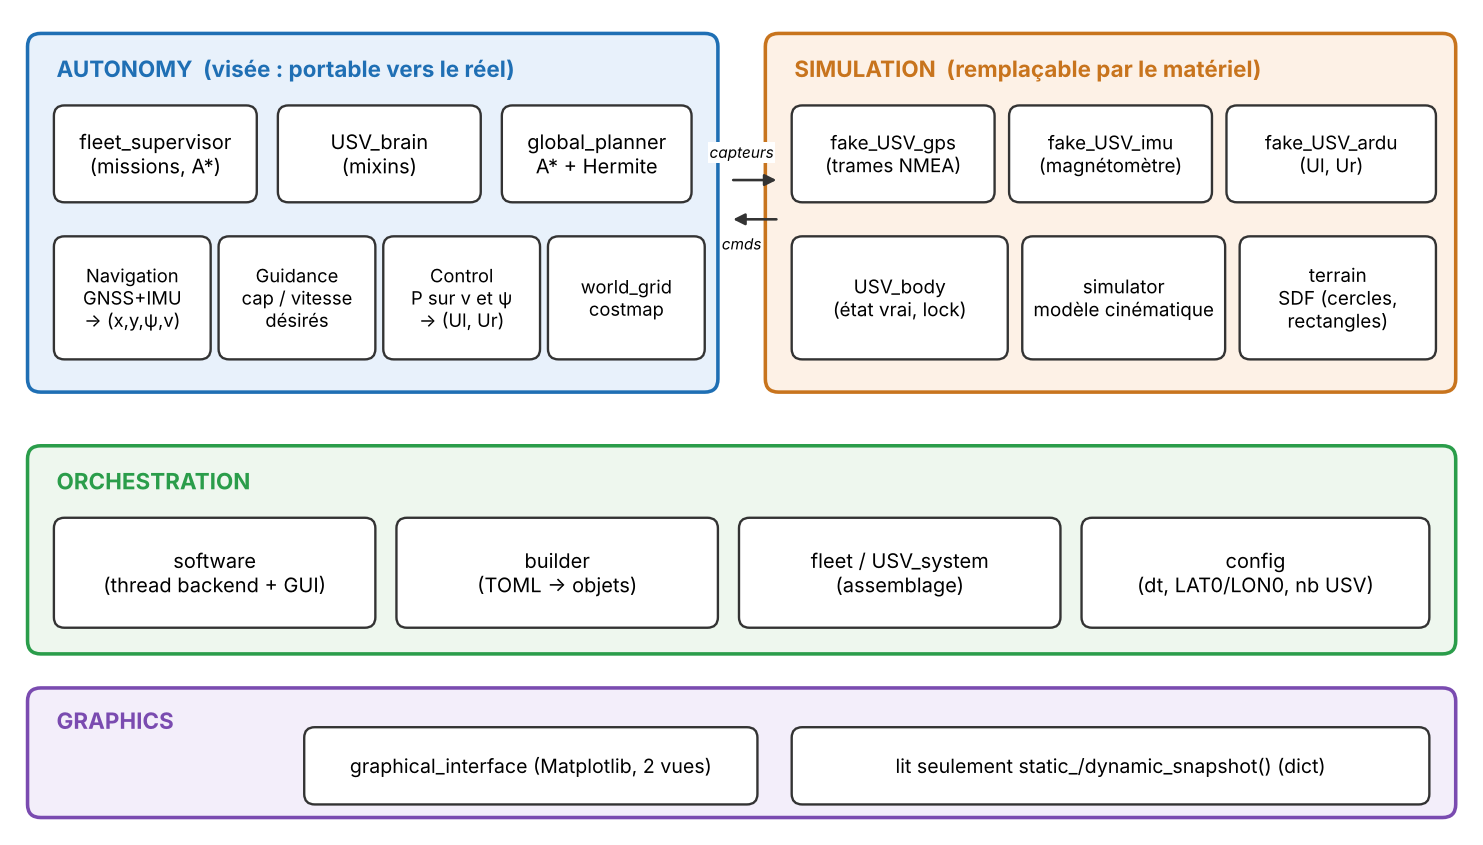
\includegraphics[width=\textwidth]{figs/architecture.png}
\caption{Architecture en couches. Le paquet \code{autonomy} est conçu pour être portable ; il dépend
encore d'une constante du paquet \code{orchestration} (voir section~\ref{sec:critique}).}
\end{figure}

\subsection{Arborescence}
\begin{lstlisting}
main.py                          point d'entree (scenario choisi en editant le fichier)
scenarios/*.toml                 4 scenarios : terrain, obstacles, mission
src/
  orchestration/                 assemblage : software, builder, fleet, config
  autonomy/                      brain (mixins), navigation, guidance, control, mission,
    guidance/                    global_planner (A*, Hermite), guidance (champ de potentiel)
    world_grid.py                grille + costmap
    fleet_supervisor.py          lance les missions et genere les chemins
  simulation/                    simulator (physique), map (terrain SDF), fleet (faux pilotes)
  graphics/graphical_interface.py   GUI Matplotlib (2 vues)
tools/plot.py                    trace du champ de potentiel (obsolete, voir section 9)
\end{lstlisting}

\subsection{Quatre décisions de conception}
\begin{description}[leftmargin=0cm,style=nextline]
\item[Pilotes factices à interface identique.] \code{USV_brain} reçoit \code{ardu}, \code{gps}, \code{imu}
par injection et ne sait pas ce qu'ils sont (typage par canard). \emph{Avantage} : remplacer les fausses
classes par de vrais pilotes série/ROS ne devrait pas toucher le cerveau. \emph{Coût} : le contrat n'est écrit nulle part
(pas de \code{Protocol} ni de classe abstraite).
\item[Vérité terrain séparée de la croyance.] Le \emph{snapshot} dynamique distingue \code{truth}
(état physique) et \code{belief} (estimation du cerveau). C'est la bonne structure pour étudier l'effet du bruit.
\emph{Limite actuelle} : sans bruit ni filtre, les deux sont quasi identiques, donc la séparation n'a pas
encore de contenu.
\item[Terrain en champ de distance signé (SDF).] Chaque forme est une fonction $(x,y)\mapsto d$ ; l'union
est un minimum. La même fonction sert à la collision, à la costmap et à l'affichage. \emph{Avantage} :
une seule source de vérité. \emph{Coût} : évaluation en $O(\text{nb de formes})$ par point.
\item[Scénarios déclaratifs (TOML) et GUI découplée.] Le terrain, les obstacles et la mission sont
décrits dans un fichier ; la GUI ne lit que des dictionnaires (\code{static_snapshot},
\code{dynamic_snapshot}). Ces dictionnaires sont déjà sérialisables, ce qui prépare une interface web par WebSocket.
\end{description}

% ------------------------------------------------------------ 4
\section{Chaîne GNC}
\begin{figure}[h]
\centering
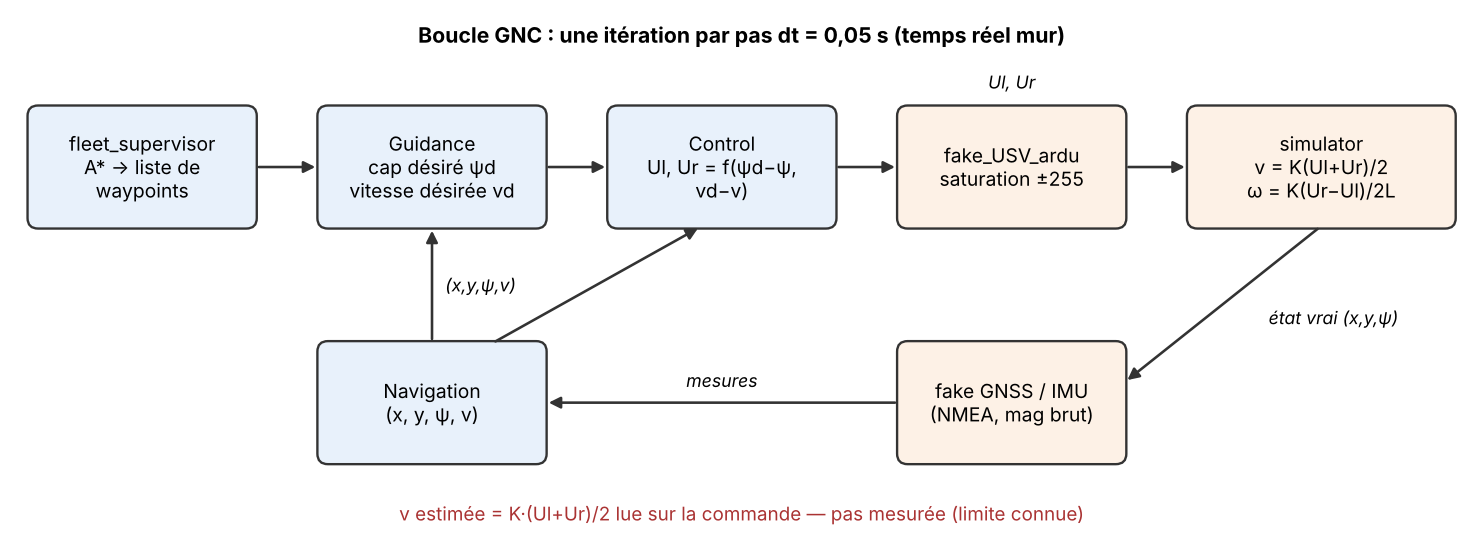
\includegraphics[width=\textwidth]{figs/gnc_loop.png}
\caption{Boucle fermée. Bleu : code d'autonomie ; orange : simulation.}
\end{figure}

\subsection{Navigation}
Le GNSS factice renvoie des trames au format NMEA (\code{ddmm.mmmm}) à partir de la position vraie ; la
navigation les convertit en degrés décimaux puis en mètres par une projection équirectangulaire autour d'un
point de référence (Paris par défaut) :
\[
x=(\lambda-\lambda_0)\,111320\cos\varphi_0,\qquad y=(\varphi-\varphi_0)\,111320 .
\]
Le cap vient du magnétomètre factice : $\psi=-\operatorname{atan2}(m_y,m_x)$. Cette approximation est
suffisante pour quelques centaines de mètres ; le code recommande lui-même \code{pyproj} à terme.
La vitesse est \emph{calculée à partir de la commande moteur} : c'est une triche assumée et listée comme
défaut majeur (section~\ref{sec:critique}).

\subsection{Guidage}
Deux modes coexistent :
\begin{itemize}
\item \textbf{Direct} (utilisé par la mission) : cap désiré = direction du waypoint courant, vitesse désirée
$v_d = 0{,}75\,v_{\max}\max(0,\cos\Delta\psi)$, ce qui ralentit le robot quand il n'est pas aligné.
\item \textbf{Champ de potentiel} (écrit, non utilisé en mission) : attraction quadratique vers le but,
répulsion autour de chaque obstacle dans un rayon $d_0=3r$, force d'attraction multipliée par 100 à moins de 20\,m du but.
\end{itemize}
Les waypoints suivis ne sont donc pas les waypoints de la mission mais ceux du chemin A* lissé
(sous-section~\ref{sec:planif}).

\subsection{Contrôle}
Régulateur proportionnel sur la vitesse et le cap, avec anticipation (\emph{feedforward}) sur la vitesse :
\begin{align*}
U_{ff}&=255\,\frac{v_d}{v_{\max}}, & U_v&=K_{p,v}\,\frac{v_d-v}{v_{\max}}, & U_\psi&=K_{p,\psi}\,\frac{\operatorname{sawtooth}(\psi_d-\psi)}{\pi},\\
U_l&=U_{ff}+U_v-U_\psi, & U_r&=U_{ff}+U_v+U_\psi,
\end{align*}
avec $K_{p,v}=5$ et $K_{p,\psi}=250$, saturés à $\pm255$ par le pilote moteur. La différence de poussée permet
de pivoter sur place. Les gains ont été trouvés par tâtonnement ; le code porte un \code{TODO} qui l'admet.

\subsection{Mission}
Une mission de type \code{go to waypoints} suit une liste dans l'ordre ; une mission \code{a_star} calcule d'abord
un chemin global vers le dernier waypoint puis le suit. Un waypoint est atteint lorsque la distance
descend sous \code{arrival_radius} ; le robot s'arrête (commandes nulles) à la fin de la liste.

% ------------------------------------------------------------ 5
\section{Planification globale}
\label{sec:planif}
\subsection{Chaîne de traitement}
\begin{enumerate}
\item \textbf{Grille} régulière à 2,5\,m de résolution couvrant l'arène, l'encoche de départ et une marge de 10\,m.
\item \textbf{Costmap} : $c=\min\!\bigl(255,\;255\,e^{-k\,d}\bigr)$ avec $d$ la distance signée à l'obstacle et
$k=\ln(255)/5\approx1{,}11\ \mathrm{m^{-1}}$. Le coût vaut 255 (bloqué) dans les obstacles et décroît jusqu'à
1 à 5\,m.
\item \textbf{A*} en 8-connexité, coût de pas $\;\text{dist}\cdot(1+w\,c)\;$ avec $w=0{,}1$,
heuristique euclidienne.
\item \textbf{Éclaircissement} : on ne garde que les points espacés d'au moins 10\,m.
\item \textbf{Lissage} par spline cubique d'Hermite (tangentes par différences centrées), 10 échantillons par segment, puis filtre à 0,5\,m.
\end{enumerate}

\subsection{Résultat mesuré}
\begin{figure}[h]
\centering
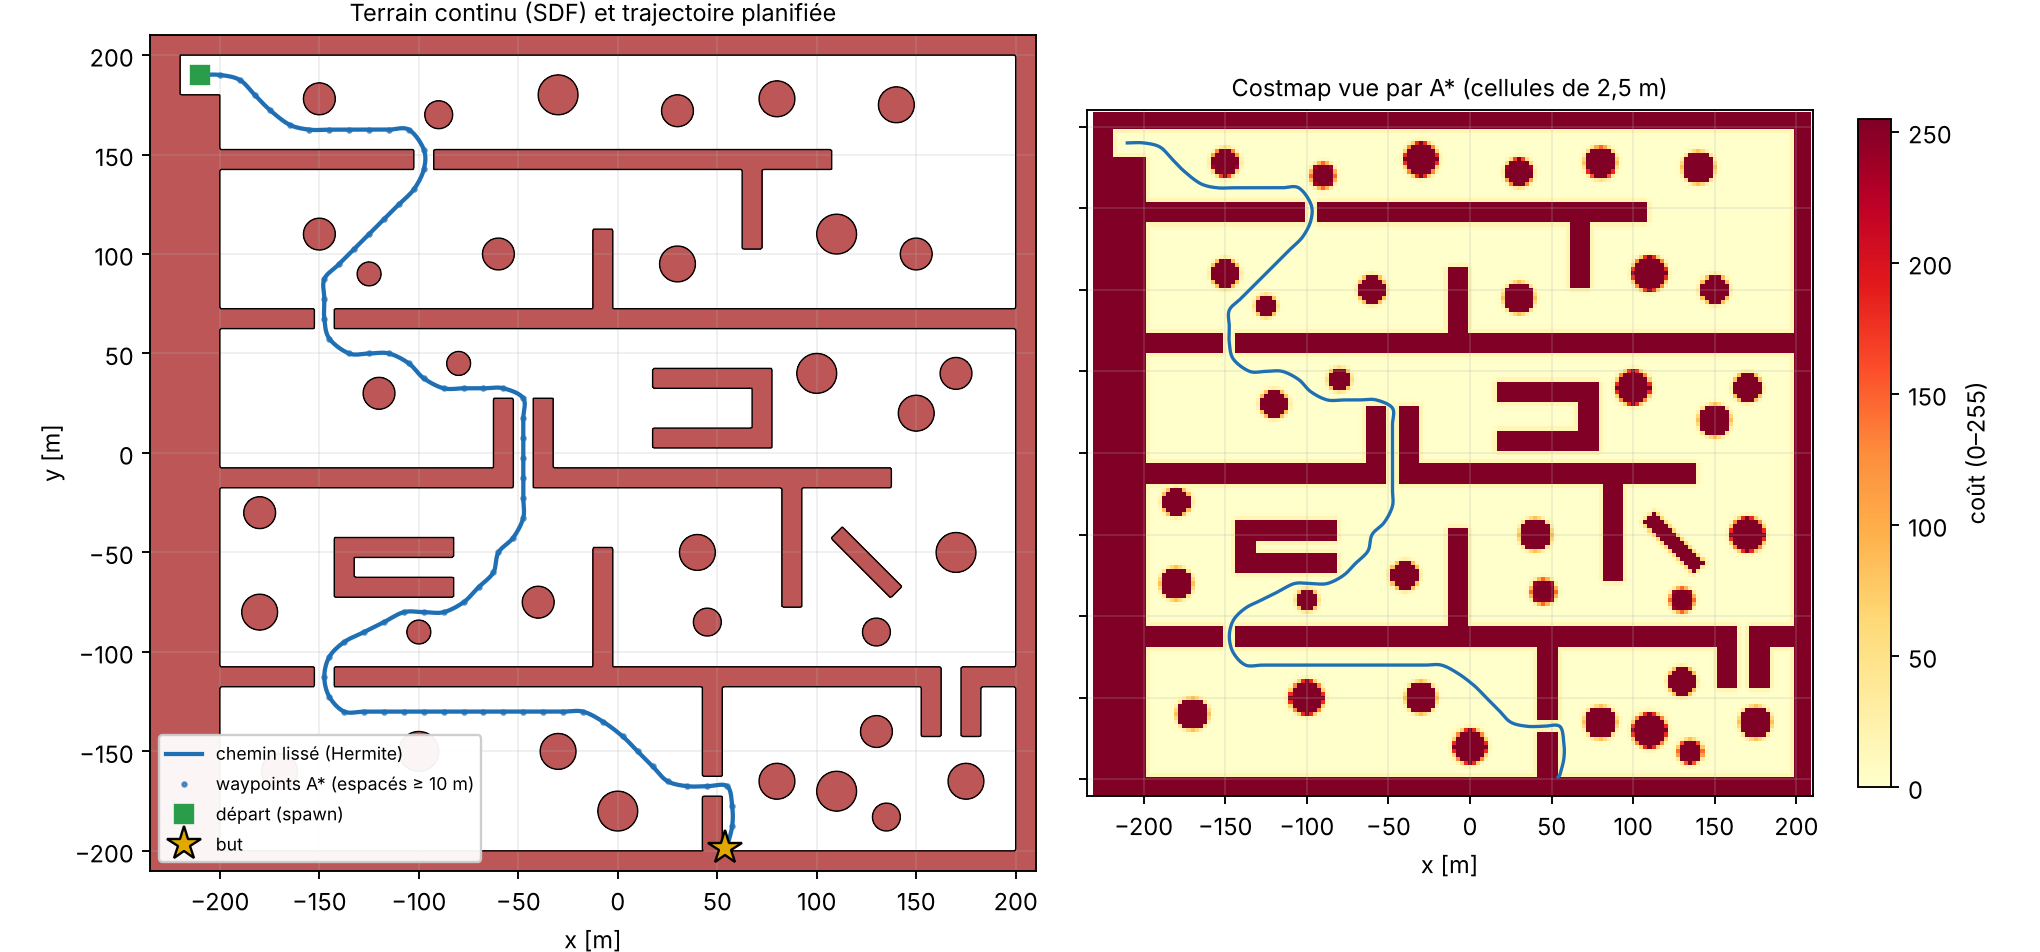
\includegraphics[width=\textwidth]{figs/scenario.png}
\caption{Scénario \code{a_star_complex} : portes étroites de 10\,m, leurres, impasses en peigne, piège en U.
Départ en haut à gauche (encoche), but en bas.}
\end{figure}

\begin{center}
\begin{tabular}{lr}
\toprule
\textbf{Grandeur (scénario \code{a_star_complex})} & \textbf{Valeur}\\
\midrule
Taille de la grille & $168\times176$ = 29\,568 cellules\\
Cellules libres (coût $<255$) & 19\,935\\
Cellules développées par A* & 17\,587 (88\,\%)\\
Temps de A* (Python pur) & 0,13\,s\\
Waypoints après éclaircissement & 78\\
Points après lissage & 695\\
Longueur du chemin lissé & 810\,m (ligne droite : 470\,m)\\
Distance minimale aux obstacles le long du chemin lissé & 1,50\,m\\
Points du chemin lissé en collision & 0\\
\bottomrule
\end{tabular}
\end{center}

\begin{note}[Comment lire ces chiffres]
Mesures faites hors du dépôt sur une reproduction fidèle des fonctions du projet (géométrie, costmap, A*, Hermite),
dans un environnement de calcul ordinaire ; les temps sont indicatifs. Le chemin ne heurte aucun obstacle sur ce scénario,
\emph{ce qui ne prouve pas que le lissage soit sûr} : rien dans le code ne vérifie la collision après lissage.
\end{note}

\subsection{Ce que ces chiffres disent de l'algorithme}
\begin{itemize}
\item Avec $w=0{,}1$, le terme de coût multiplie le pas jusqu'à $\times26$ près des obstacles. A* développe 88\,\% des cellules libres :
il se comporte presque comme un Dijkstra. C'est acceptable en 2D à cette taille ; ce ne le sera pas en 3D.
\item Seules les cellules à $d\le0$ sont bloquées : il n'y a pas d'inflation par la taille du véhicule. La marge de 1,5\,m observée
vient du coût exponentiel, pas d'une garantie.
\item Les diagonales ne vérifient pas le franchissement de coin entre deux cellules bloquées.
\end{itemize}

% ------------------------------------------------------------ 6
\section{Simulation}
\subsection{Modèle physique}
Modèle cinématique idéal à commande différentielle, avancé à pas fixe $\Delta t=0{,}05$\,s :
\[
v=K\,\frac{U_l+U_r}{2},\quad \omega=K\,\frac{U_r-U_l}{2L},\quad
x\leftarrow x+v\cos\psi\,\Delta t,\quad y\leftarrow y+v\sin\psi\,\Delta t,\quad \psi\leftarrow\psi+\omega\,\Delta t,
\]
avec $K=v_{\max}/255$, $v_{\max}=6$\,m/s, $L=1$\,m. Les constantes $K$ et $L$ sont arbitraires.
Il n'y a ni inertie, ni traînée, ni courant, ni vent : la vitesse suit la commande instantanément.

\subsection{Collisions}
Si la position suivante est dans un obstacle (distance signée $<0$), le pas est annulé \emph{en bloquant aussi la rotation} :
un robot qui touche un obstacle reste figé définitivement. C'est un comportement de détection, pas de récupération.

\subsection{Threads}
Un thread de fond exécute à chaque pas : mission, puis physique, puis attend pour tenir $\Delta t$ en temps mural.
La GUI tourne dans le thread principal et rafraîchit chaque $\Delta t$. La simulation est donc \emph{liée à l'horloge murale} :
elle ne peut pas aller plus vite que le temps réel et n'est pas déterministe.

% ------------------------------------------------------------ 7
\section{Interface graphique}
La GUI affiche deux vues synchronisées en zoom : le terrain continu (SDF) et la costmap discrète telle que A*
la voit. Pour chaque robot : position vraie (flèche de cap), position estimée (croix), trace parcourue,
chemin planifié et cible courante. Elle ne consomme que deux fonctions renvoyant des dictionnaires.
C'est la partie réalisée avec le plus d'aide de l'IA (section~\ref{sec:ia}). Limites : Matplotlib
n'est ni conçu pour du 3D interactif ni pour des dizaines de robots temps réel, et la GUI ne permet aucune entrée utilisateur.

% ------------------------------------------------------------ 8
\section{Scénarios fournis}
\begin{center}
\begin{tabularx}{\textwidth}{l c c c c X}
\toprule
\textbf{Fichier} & \textbf{Arène} & \textbf{Cercles} & \textbf{Rect.} & \textbf{WP} & \textbf{Remarque}\\
\midrule
\code{direct_waypoints} & $\pm25$\,m & 0 & 0 & 12 & Suivi direct, rayon 0,25\,m\\
\code{obstacle_avoidance} & $\pm50$\,m & 15 & 1 & 8 & \textbf{Ne démarre pas} : clé \code{type} absente\\
\code{a_star} & $\pm200$\,m & 26 & 14 & 1 & Murs, piège en U, barre à 45\textdegree\\
\code{a_star_complex} & $\pm200$\,m & 34 & 26 & 1 & Pire cas voulu : portes de 10\,m = 2 cellules\\
\bottomrule
\end{tabularx}
\end{center}

% ------------------------------------------------------------ 9
\section{Installation et lancement}
\begin{lstlisting}
git clone <repository-url>
cd Tactical-Navigation
uv sync
uv run python main.py
\end{lstlisting}
Prérequis : Python 3.13 ou plus récent, \code{uv}, un backend graphique Matplotlib (Tk ou Qt ; sous Ubuntu : \code{python3-tk}).
Le scénario se choisit \textbf{en modifiant} \code{main.py} (pas d'option en ligne de commande).

\begin{verdict}[Avertissement : le README du dépôt est périmé]
Il décrit encore \code{launch.py}, des paramètres \code{dict_of_waypoints} dans \code{config.py}, des missions \code{wpts}/\code{test}
et un thread de mission par USV. Aucun n'existe dans le code actuel. Le champ de potentiel y est présenté comme la fonctionnalité centrale
alors que la mission utilise désormais A* et un guidage direct. Se fier à ce document, pas au README.
\end{verdict}

% ------------------------------------------------------------ 10
\section{Évaluation critique}
\label{sec:critique}
\subsection{Ce qui est solide}
\begin{itemize}
\item Séparation cerveau / pilotes par injection : la bonne direction pour passer au matériel ou à ROS.
\item Terrain SDF unifié (collision, costmap, affichage) et scénarios déclaratifs : ajouter un terrain coûte un fichier.
\item Distinction vérité / croyance dans les snapshots, et snapshots sérialisables.
\item Échelle de test pertinente : le scénario complexe contient de vrais leurres et impasses, pas un labyrinthe trivial.
\item Les limites du modèle sont écrites dans le code (\code{TODO}) et le README : la dette est connue.
\end{itemize}

\subsection{Défauts vérifiés à la lecture du code}
Chaque ligne ci-dessous a été relevée dans le code fourni.

\begingroup\small
\begin{longtable}{>{\raggedright\arraybackslash}p{0.5cm}>{\raggedright\arraybackslash}p{9.6cm}>{\centering\arraybackslash}p{1.6cm}}
\toprule
\textbf{\#} & \textbf{Constat} & \textbf{Gravité}\\
\midrule
\endhead
1 & \code{obstacle_avoidance.toml} n'a pas de clé \code{type} : \code{fulfill_mission} lève une \code{KeyError} dans le thread de fond.
Le thread meurt, la fenêtre reste ouverte et immobile, sans message clair. & \haute\\
2 & Simulation liée à l'horloge murale : pas d'exécution accélérée, pas de reproductibilité. Bloquant pour les tests, les \emph{benchmarks}
et surtout l'apprentissage par renforcement visé par le projet. & \haute\\
3 & README périmé (voir section 9). & \haute\\
4 & Accès concurrent : \code{dynamic_snapshot()} appelle \code{brain.get_nav_state()} depuis le thread GUI ; cette méthode
\emph{modifie} l'état du cerveau pendant que le thread de fond l'utilise. & \moyenne\\
5 & La vitesse « estimée » est lue sur la commande avec $K$ connu : la navigation ne fait aucune estimation réelle, vérité $\approx$ croyance.
Aucun bruit sur GNSS/IMU. & \moyenne\\
6 & Superviseur codé en dur (\code{"usv1"}, premier asset) alors que \code{nb_of_USVs} est paramétrable. Le multi-USV n'est pas supporté. & \moyenne\\
7 & Collision $\Rightarrow$ le robot est figé définitivement (position et cap non mis à jour). & \moyenne\\
8 & Évitement local absent de la mission : le guidage direct est actif, le champ de potentiel est en commentaire. Un obstacle non cartographié n'est pas évité. & \moyenne\\
9 & Lissage d'Hermite sans test de collision ; pas d'inflation par la taille du robot ; franchissement de coin en diagonale non vérifié. & \moyenne\\
10 & Force répulsive du champ de potentiel avec des exposants empiriques (0,75 et 2,75) : ce n'est pas le gradient du potentiel $U$ affiché.
La surface 3D de \code{tools/plot.py} est donc indicative. & \moyenne\\
11 & \code{tools/plot.py} lit \code{parameters["dict_of_waypoints"]}, absent de \code{config.py} : le script plante si on ne passe pas les dictionnaires. & \moyenne\\
12 & Cerveau en héritage multiple de quatre \emph{mixins} qui utilisent \code{self.ardu}, \code{self.max_speed}, \code{self.current_heading()}
sans les déclarer : contrat implicite et fragile. & \moyenne\\
13 & Couplages inverses : \code{autonomy/utils.py} importe \code{orchestration.config} ; \code{simulation/.../USV.py} importe \code{autonomy.brain} (inutilisé). & \moyenne\\
14 & Costmap calculée par double boucle Python : environ 7,6\,s contre 0,05\,s en version vectorisée (même résultat à $3\times10^{-14}$ près) sur le scénario complexe.
La fonction \code{distance} accepte déjà des tableaux NumPy. & \basse\\
15 & Le nom du scénario (clé racine du TOML) n'est pas transmis : \code{build_mission} ne garde que la section \code{[mission]}, le titre de la GUI est vide. & \basse\\
16 & Test intégré de \code{global_planner.py} (\code{\_\_main\_\_}) appelle \code{A_star} avec une mauvaise signature ; \code{local_planner.py} est vide ;
\code{terrain.gradient} divise par une norme qui peut être nulle. & \basse\\
17 & Aucun test automatisé, aucune CI ; \code{.gitignore} ne contient que \code{.venv} ; \code{\_\_init\_\_.py} seulement à la racine de \code{src}. & \basse\\
18 & Style : classes en minuscules (\code{terrain}, \code{simulator}, \code{software}), mélange français/anglais, fautes dans des noms (\code{lenght}). & \basse\\
\bottomrule
\end{longtable}
\endgroup

\subsection{Risques structurels pour la suite}
\begin{description}[leftmargin=0cm,style=nextline]
\item[Passage à l'échelle (multi-robots, 3D).] La grille de coûts 2D, le terrain SDF 2D et une simulation en Python pur
n'iront pas tels quels vers un terrain 3D avec plusieurs types de robots. Une grille 3D à 2,5\,m multiplie les cellules par le nombre de couches, et A* en 88\,\% d'exploration
ne suit pas. Le choix « un seul outil du début à la fin » est donc un pari, pas un acquis.
\item[Apprentissage par renforcement.] Il exige un pas de simulation rapide, déterministe et indépendant de l'affichage.
L'architecture actuelle n'a aucune de ces trois propriétés.
\item[Réalisme.] Un modèle sans inertie rend n'importe quel contrôleur proportionnel acceptable. Les faiblesses du contrôle n'apparaîtront
qu'avec une dynamique plus réaliste, ce que la feuille de route prévoit mais qui n'est pas commencé.
\end{description}

% ------------------------------------------------------------ 11
\section{Feuille de route}
\label{sec:roadmap}
Ordre proposé, du plus structurant au plus cosmétique. La liste d'origine du projet est conservée, réordonnée selon les risques ci-dessus.

\begin{center}
\begin{tabularx}{\textwidth}{c >{\raggedright\arraybackslash}p{4.4cm} X}
\toprule
\textbf{Priorité} & \textbf{Chantier} & \textbf{Pourquoi}\\
\midrule
1 & Découpler pas de simulation, horloge murale et GUI ; graine aléatoire & Reproductibilité, tests, RL, vitesse\\
2 & Corriger les défauts 1, 3, 4, 6 & Le dépôt doit se lancer et se lire sans surprise\\
3 & Premiers tests unitaires (géométrie SDF, A*, conversions, contrôleur) & Filet de sécurité avant de refactorer\\
4 & Isoler \code{autonomy} de la simulation (contrats explicites, plus de mixins implicites) & Condition de la portabilité promise\\
5 & Bruit capteurs, estimation de vitesse, puis filtre (EKF) & Donne un contenu à « vérité vs croyance »\\
6 & Dynamique plus réaliste, contrôleur PID, réglage des gains & Révèle les faiblesses du contrôle\\
7 & Évitement local (capteur de distance simulé, costmap locale) & Réagir à l'imprévu\\
8 & Machine à états, multi-USV, ordonnancement (plus proche voisin) & Missions enchaînées, coordination\\
9 & Interface web par WebSocket, puis 3D & Seulement après 1 à 5\\
\bottomrule
\end{tabularx}
\end{center}

\subsection*{Décisions ouvertes}
\begin{center}
\begin{tabularx}{\textwidth}{>{\raggedright\arraybackslash}p{3.1cm}XX}
\toprule
\textbf{Option} & \textbf{Pour} & \textbf{Contre}\\
\midrule
Noyau Python + NumPy, points chauds vectorisés & Rapide à écrire ; l'existant continue de servir & Plafond de performance en 3D multi-robots\\
Noyau Python + module C++ (liaison) pour A* et la physique & Gros gain de vitesse ciblé ; valorise le C++ & Deux langages à maintenir\\
ROS\,2 + simulateur existant & Écosystème, proche du réel & Courbe d'apprentissage, simulation moins contrôlable pour le RL\\
\bottomrule
\end{tabularx}
\end{center}
Aucune option n'est tranchée dans ce document : la décision dépend de la taille visée (nombre de robots, 3D, RL) et doit venir après le chantier 1.

% ------------------------------------------------------------ 12
\section{Rôle de l'IA dans le projet}
\label{sec:ia}
Transparence sur la contribution d'un assistant IA (Claude, Anthropic) :
\begin{itemize}
\item selon le README du dépôt, le code de l'interface graphique et du script de tracé a été obtenu avec son aide ;
\item l'assistant est utilisé comme superviseur technique : présenter des options avec avantages et inconvénients,
challenger les choix, relire l'architecture, sans écrire le projet à la place de l'auteur ;
\item ce document, ses figures, ses mesures et la revue critique de la section~\ref{sec:critique} ont été produits avec cette assistance
à partir du code source fourni.
\end{itemize}
Les choix algorithmiques et leur justification restent à défendre par l'auteur.

% ------------------------------------------------------------ A
\appendix
\section{Inventaire des modules}
\begin{center}
\small
\begin{tabularx}{\textwidth}{>{\raggedright\arraybackslash}p{6.7cm}X}
\toprule
\textbf{Module} & \textbf{Rôle}\\
\midrule
\code{orchestration/software.py} & Démarre le thread de fond, la GUI, construit les snapshots\\
\code{orchestration/builder.py} & Charge un TOML, construit terrain, mission, flotte\\
\code{orchestration/fleet.py} & Regroupe cerveau, corps et pilotes d'un robot\\
\code{orchestration/config.py} & $\Delta t$, nombre d'USV, point de référence géodésique\\
\code{autonomy/brain.py} & Cerveau : héritage de mission, guidage, navigation, contrôle\\
\code{autonomy/navigation.py} & GNSS/IMU vers $(x,y,\psi,v)$\\
\code{autonomy/guidance/guidance.py} & Cap direct, champ de potentiel, vitesse désirée\\
\code{autonomy/control.py} & Régulateur proportionnel avec anticipation\\
\code{autonomy/mission.py} & Pas de suivi de waypoint, test de mouvement\\
\code{autonomy/world_grid.py} & Grille régulière et costmap exponentielle\\
\code{autonomy/guidance/global_planner.py} & A* 8-connexe pondéré, lissage d'Hermite\\
\code{autonomy/fleet_supervisor.py} & Choisit le type de mission, génère le chemin global\\
\code{simulation/simulator.py} & Physique cinématique, détection de collision\\
\code{simulation/map/geometry.py} & SDF : cercle, rectangle tourné, polygone, union\\
\code{simulation/map/terrain.py} & Arène, encoche de départ, murs, distance, tracé\\
\code{simulation/fleet/hardware/*} & Faux GNSS (NMEA), faux IMU, faux contrôleur moteur\\
\code{simulation/fleet/vehicles/USV.py} & État vrai du USV protégé par un verrou\\
\code{graphics/graphical_interface.py} & GUI Matplotlib à deux vues\\
\code{tools/plot.py} & Trace du champ de potentiel (obsolète)\\
\bottomrule
\end{tabularx}
\end{center}

\section{Méthode des mesures}
Les valeurs de la section~\ref{sec:planif} et le défaut n\textdegree14 ont été obtenus en exécutant, hors du dépôt,
des copies des fonctions \code{circle}, \code{rectangle}, \code{polygon}, \code{union}, de la formule de costmap, de \code{A_star}
et de \code{smooth_path_with_hermite_spline}, sur les données de \code{a_star_complex.toml}. Départ : $(-210;190)$, but : $(54;-198{,}5)$,
résolution 2,5\,m, marge 10\,m. Le temps de la costmap compare la double boucle d'origine et une évaluation vectorisée de la même formule.
La distance minimale est l'évaluation de la SDF en chaque point du chemin lissé. Les valeurs de temps dépendent de la machine ;
les nombres de cellules, de waypoints et de points sont déterministes.

\end{document}
